\documentclass[twoside,12pt,a4paper]{scrreprt}
\usepackage[T1]{fontenc}
\usepackage[utf8]{inputenc}
\usepackage[ngerman]{babel}
\usepackage{babelbib}
\usepackage{parskip}
\usepackage{microtype}
\usepackage{graphicx} % Zum Einbinden von Grafiken
\usepackage[dvipsnames]{xcolor}
\usepackage[colorlinks=true,linkcolor=Black,citecolor=MidnightBlue,urlcolor=MidnightBlue]{hyperref}
\usepackage[all]{hypcap}
\usepackage{pgfplots} \pgfplotsset{compat=1.9}
\usepackage{helvet} % Schönere SansSerif-Schrift
\usepackage{times}  % Schönere Serif-Schrift

\usepackage{blindtext} % sollte am Ende nicht mehr benötigt werden ;)

\pagestyle{headings}

\graphicspath{ {figures/} } % Pfad-Prefix für einzubindende Grafiken. Es sind auch mehrere Pfade möglich, diese müssen jeweils in eigenen {Klammern} stehen.

\setkomafont{disposition}{\normalcolor\bfseries} % überall Serifen verwenden
% oder
%\renewcommand{\familydefault}{\sfdefault} % überall Sans-Serif verwenden

% PDF-Optionen (werden in den Dateieigenschaften angezeigt)
\hypersetup{
pdftitle={Entwicklung einer Webanwendung zur Annotation spezifischer linguistischer Merkmale in Fließtexten},
pdfauthor={Oliver Brehm},
pdfsubject={Masterarbeit Infromatik},
pdfpagelayout=TwoColumnRight
}

%%% Eigene Makros
\newcommand{\qq}[1]{\glqq #1\grqq} % \qq{Text in Anführungszeichen}

\begin{document}

%%% Titelseite
\begin{titlepage}
\begin{center}
\LARGE Eberhard Karls Universität Tübingen\\
\large Mathematisch-Naturwissenschaftliche Fakultät \\
Wilhelm-Schickard-Institut für Informatik\\
[3cm]
\huge Masterarbeit Informatik\\
[2cm]
\Large\textbf{Entwicklung einer Webanwendung zur Annotation spezifischer linguistischer Merkmale in Fließtexten}\\
[1.5cm]
\large Oliver Brehm\\
[0.5cm]
31.01.2017\\
\vfill
\small\textbf{Gutachter}\\[0.3cm]
\large Jun.-Prof. Dr. Alexandra Kirsch\\
\footnotesize Wilhelm-Schickard-Institut für Informatik\\Universität Tübingen\\
[1cm]
\small\textbf{Betreuer}\\[0.3cm]
\large M.Sc. Heiko Holz\\
\footnotesize Wilhelm-Schickard-Institut für Informatik\\Universität Tübingen
\end{center}
\end{titlepage}

%%% Titelrückseite: Bibliographische Angaben
\thispagestyle{empty}
\vspace*{\fill}
\textbf{Brehm, Oliver:}\\
\emph{Entwicklung einer Webanwendung zur Annotation spezifischer linguistischer Merkmale in Fließtexten}\\
Masterarbeit Informatik\\
Eberhard Karls Universität Tübingen\\
Bearbeitungszeitraum: August 2017 - Januar 2018
\newpage

%%% Zusammenfassung (Abstract), hier aus externer Datei eingebunden
% !TEX root = ../ausarbeitung.tex

\begin{abstract}
\section*{Zusammenfassung}

Viele Menschen haben Schwierigkeiten, flüssig zu Lesen und zu Schreiben. Man spricht von einer Lese- Rechtschreibschwäche (LRS), wenn keine erkennbaren äußeren Umstände (wie soziales Umfeld, oder längerer Schulausfall z.B. durch Krankheit) die Entwicklung der Lese- und Schreibkompetenz beeinträchtigen. Es wurde gezeigt, dass gezielte Übungen wie das Erfassen von Silben und Sprachrhythmus dazu führen können, diese Fähigkeiten zu verbessern. In der Therapie werden häufig Übungstexte verwendet, in denen Silben abwechselnd in verschiedenen Schriftfarben dargestellt werden.

In dieser Arbeit wurde eine Web-Applikation entwickelt, mit der es ermöglicht werden sollte, solche farblich markierten Texte einfach und automatisch zu erstellen. Für die Verdeutlichung des Sprachrhythmus sollte auch die betone Silbe im Wort speziell markiert werden können. Es wurde zunächst untersucht, wie aus einem beliebigen Text automatisch Silbentrennung und Wortbetonung bestimmt werden können. Dazu wurde eine, auf einem Lexikon basierende Datenbank aufgebaut, die für jedes Wort diese Merkmale enthält. Die Datenbank ist durch NutzerInnen der Anwendung erweiterbar, hinzugefügte Einträge müssen jedoch von ExpertInnen oder anderen NutzerInnen verifiziert werden, damit sie global verfügbar sind. Für die Applikation wurden zunächst die Anforderungen analysiert und anschließend zwei Hauptkomponenten entwickelt: Auf der einen Seite das Backend, welches Anfragen der Web-Applikation, wie z.B. den zu analysierenden Text entgegen nimmt und beantwortet, sowie die erstellte Wortdatenbank und eine weitere Datenbank, die nutzerspezifische Einstellungen speichert, verwaltet. Auf der anderen Seite steht die Entwicklung des Frontends, der eigentlichen Web-Applikation, welche mit NutzerInnen interagiert, Anfragen an das Backend schickt und die dadurch erhaltenen Informationen entsprechend darstellt.

Die abschließende Evaluation zeigt, dass die Applikation Übungstexte erfolgreich erstellen kann. Mit einem Nutzertest wurde festgestellt, dass die meisten Anwendungsfälle in der Web-Oberfläche intuitiv und zeiteffizient durchgeführt werden konnten. Die erkannten Probleme können durch eine Überarbeitung der Nutzeroberfläche mit wenig Aufwand behoben werden. Weitere Anmerkungen der ProbandInnen generierten interessante, weiterführende Ideen, die auf diese Arbeit aufbauend gut realisierbar sind.

\end{abstract}
\newpage

%%% Inhaltsverzeichnis
\KOMAoption{toc}{listof,bib} % Abbildungs-/Tabellenverzeichnis, Literaturverzeichnis aufnehmen
\tableofcontents\label{toc}
\cleardoublepage

%%% Hauptteil (mit \input{dateiname} wird die Datei 'dateiname' eingebunden)
% !TEX root = ../ausarbeitung.tex

\chapter{Einleitung}

In der vorliegenden Arbeit wurde eine Applikation entwickelt, die Fließtexte durch farbliche Annotationen so aufbereiten kann, dass diese als Übungstexte in der Therapie von Kindern mit Lese-Rechtschreibschwäche (LRS) eingesetzt werden können. Solche Übungstexte werden häufig von LerntherapeutInnen manuell, z.B. mit einem Textverarbeitungsprogramm mit viel Aufwand erstellt. Die Zielgruppe für die Benutzung der Applikation sind also LerntherapeutInnen, Lehrkräfte oder auch die Eltern betroffener Kinder, deren Arbeit durch die Automatisierung des Prozesses der Erstellung von Übungstexten erleichtert werden kann.\\

LRS tritt bei ca. 700000 Kindern und Jugendlichen unter 18 Jahren auf \cite{Schulte-Koerne2014} \todo{andere zahlen, andere quelle}. Bei der Therapie gibt es verschiedene Maßnahmen um die Lese- und Schreibkompetenz von Betroffenen zu fördern. Das Lesen speziell bearbeiteter Texte zielt z.B. darauf ab, die Dekodierfähigkeit zu verbessern, deren Unterentwicklung neben anderen Faktoren einen Teil der Ursachen für LRS abdeckt\cite{Schulte-Koerne2014}. Es wurde gezeigt, dass beim fortgeschrittenen Lesen und Schreiben nicht Buchstaben und Laute die erfassten Elemente sind, sondern größere orthographische Einheiten, wie Silben oder ganze Wörter\cite{Steinbrink2014}. Eine Zentrale Rolle spielt dabei das Erkennen von Silben. Die Silbenmethode und Silbenfibeln sind beim Schrifterwerb im schulischen Umfeld im Einsatz \todo{seit wann?} und können Erfolge aufweisen\tocite{Silbenmethode, einsatz, Bredel, Tophinke}. Eine weitere Erkenntnis hat gezeigt, dass die Wahrnehmung von Sprachrhythmus ebenfalls eine Auswirkung auf die Lese- und Schreibkompetenz hat\cite{Brandelik2014}. Es wird vermutet, dass ein gezieltes Training der Bewusstheit von Silbenbetonung zu höherem Lernerfolg führen kann\cite{Holz2017} (s. Abschnitt \ref{sec:dekodierung}). Im Folgenden Kapitel werden auch einige Alternativen vorgestellt, die das Lesen Lernen mit der Silbenmethode unterstützen.\\
Basierend auf diesen Überlegungen wurde die Applikation mit der Motivation entwickelt, das Erstellen von Übungstexten zu vereinfachen und zu automatisieren. In den Übungstexten werden Wörter in Silben unterteilt, welche sich mit verschiedenen Farben hervorheben lassen. Im Gegensatz zu ähnlichen Ansätzen (sowohl Lehrmaterial in Papierform als auch digitale Ansätze) bietet die Applikation zusätzlich die Möglichkeit, die betonte Silbe im Wort besonders (z.B. in einer anderen Farbe) darzustellen. Weitere Merkmale, wie der Abstand zwischen Silben und Wörtern, sowie ein Silbentrennzeichen, lassen sich frei anpassen. Die Anwendung kann LerntherapeutInnen, Lehrkräften oder Eltern helfen, spezifisch zugeschnittene Übungen mit wenig Aufwand selbst zu erstellen.\\

Es können viele Gründe genannt werden, weshalb wir uns von der Entwicklung einer solchen Anwendung Erfolg versprachen: Ein Grund ist die effizientere Nutzung von Ressourcen. Automatisierung von Aufgaben bringt immer einen Zeitgewinn für die Personen, die diese sonst erledigen mit sich. Zeit, welche die LerntherapeutInnen beim Erstellen von Übungsmaterial einsparen, kann z.B. für eine Bessere Vorbereitung der Therapie oder zu mehr Betreuungszeit von SchülerInnen führen. Außerdem ist die Gestaltung von Übungsmaterial sehr flexibel, da in der Software viele Einstellungen für die Textdarstellung vorgenommen werden können. So können die LerntherapeutInnen einfach verschiedene Möglichkeiten beim Erstellen von Übungstexten ausprobieren und bei der Verwendung mit den SchülerInnen deren Präferenzen erkennen. Dadurch lassen sich eventuell direkt Erkenntnisse gewinnen, welche Art von Textannotation am besten funktioniert.\\
Bei der Recherche konnte nur wenig vergleichbare Software gefunden werden. Tools, die ebenfalls die Aufgabe der Annotation von Silben in Texten erledigen sind zum Teil veraltet oder bieten wenig Möglichkeiten zur Anpassung der Annotation (s. Abschnitt \ref{sec:lrs-digital}).

Die Entwicklung der Anwendung stellte verschiedene Herausforderungen in diversen Bereichen dar. Zuerst musste untersucht werden, wie in Wörtern Silbentrennung und Wortbetonung automatisch bestimmt werden kann. Hierfür wurde eine eigene Datenbank aufgebaut, die diese und andere Merkmale speichert. Eine besondere Schwierigkeit stellte die Komplexität und der Umfang der deutschen Sprache dar. Als Grundlage für die Datenbank diente das Lexikon CELEX2\cite{Burnage1990}, aus dem rund 360 000 Einträge, welche sowohl aus Grund- als auch Flexionsformen von Wörtern bestehen, extrahiert werden konnten. Damit ist es aber nicht möglich den deutschen Wortschatz lückenlos mit allen Flexionsformen abzubilden. Es wurde deshalb nach einer Möglichkeit gesucht, eine benutzerfreundliche Schnittstelle zu bieten, mit der korrekte Einträge von NutzerInnen und Experten manuell, mit wenig Aufwand der Datenbank hinzugefügt werden können. Es wurde untersucht, welche Ansätze es gibt, mit \textit{Croudsourcing} die Erweiterbarkeit der Datenbank auf die NutzerInnen aufzuteilen (s.Abschnitt \ref{sec:forschung-database}). So könnten beispielsweise auch Eigennamen, die in als Übungstexte verwendeten Geschichten häufig auftauchen, Teil des Wortschatzes werden.\\

Vor der Entwicklungsphase mussten der Rahmen und Funktionsumfang der Software definiert und die einzelnen Komponenten spezifiziert werden. Dafür wurde zunächst eine Anforderungsanalyse durchgeführt. Hierbei wurden Ideen aus verschiedenen Quellen gesammelt, es wurden Brainstormings in der eigenen Forschungsgruppe durchgeführt, sowie Gespräche mit ExpertInnen aus der Computerlinguistik und der Lerntherapie geführt. Alle wichtigen Aspekte der Applikation wie Design, Arten der Textannotation, Funktionen der Wortdatenbank und des Nutzerkontos etc. wurden diskutiert. So entstanden viele Ideen und Szenarien woraus dann eine Spezifikation erarbeitet werden konnte. In einer späteren Phase der Entwicklung entstanden parallel noch weiter Ideen für Features, die am Anfang nicht vorgesehen waren. Daher wurden die ins Projekt involvierten Personen zusätzlich mit einem Fragebogen gebeten, die Wichtigkeit weiterer Features zu bewerten und anzugeben mit welcher Priorität diese noch entwickelt werden sollten.\\
Einen wichtigen Punkt für die Entwicklung der Webapplikation stellte die User Experience dar. Die Zielgruppe der Nutzer, welche die Applikation letztendlich bedienen sollen, wurde auf LerntherapeutInnen, Lehrkräfte und Eltern von Betroffenen Kindern festgelegt. Diese bringen sehr unterschiedliche Kenntnisse im Umgang mit Software bzw. Webanwendungen mit. Haben die NutzerInnen Schwierigkeiten, das Programm zu bedienen, führt das schnell zu Frust und letztendlich dazu, dass die Software am Ende überhaupt nicht genutzt, und die Aufgabe weiterhin manuell erledigt wird. \tocite{User Experience wichtig} Das Ziel war also die Oberfläche so einfach und intuitiv wie möglich zu gestalten, um Allen NutzerInnen einen reibungslosen Umgang mit der Applikation zu ermöglichen. Es wurde beschlossen eine Webbrowser-basierte Anwendung zu entwickeln, welche plattformunabhängig funktioniert. Damit wurden von Anfang an Hürden, wie die Bindung an ein bestimmtes Betriebssystem und die Notwendigkeit der Installation von Software beseitigt. Die Applikation kann von jedem Computer mit Internetverbindung und Webbrowser sofort benutzt werden. Durch die Verwendung von Nutzerkonten sind nutzerspezifische Einstellungen überall gleichermaßen abrufbar.\\

Im Evaluationsteil am Ende der Arbeit wurde die Benutzbarkeit des Gesamtsystems anhand eines Nutzertests bewertet. Hierfür wurden als ProbandInnen sowohl Experten (Lerntherapeutinnen) als auch Laien herangezogen. Für Auswahl der ProbandInnen aus der Gruppe der Laien gab es keine Beschränkungen, da in der Zielgruppe auch Elternteile von betroffenen LRS Kindern enthalten sind und diese aus den verschiedensten Berufsfeldern sowie unterschiedlichen Altersgruppen stammen können. Zunächst wurde ein Pilottest ausgeführt, um Mängel im Design des Tests, sowie Fehler der Webanwendung, die nicht im Zusammenhang mit der Usability standen im Vorfeld zu finden und zu beheben. Im Anschluss wurde der Nutzertest mit sieben ProbandInnen ausgeführt und die Ergebnisse zusammengetragen und bewertet.\\

In den Folgenden Kapiteln werden zunächst die Grundlagen zur Lese-Rechtschreibschwäche, sowie zu linguistischen Begriffen und Technologien erklärt. Danach wird der Prozess der Planung und Entwicklung der Software beschrieben. Detaillierte Beschreibungen zu einzelnen Komponenten und zum Zusammenspiel dieser sollen verdeutlichen, wie das System funktioniert. Den Abschluss der Arbeit bildet die Evaluation anhand von Beispielen mit der Applikation produzierter Texte und der Beschreibung und Durchführung des Nutzertests. Hier wird gezeigt, wie der entwickelte Prototyp im tatsächlichen Einsatz zu bewerten ist. Die Evaluation zeigt sowohl Stärken als auch Schwächen des Systems auf, die in einem weiteren Einsatz noch zu beheben sind. Die Flexibilität des Gesamtsystems schaffte zudem viele anregende neue Ideen, die im Anschluss an diese Arbeit gut realisierbar sind.
\cleardoublepage

% !TEX root = ../ausarbeitung.tex

\chapter{Stand der Forschung}

Die Motivation der Arbeit beruht auf Erkenntnissen zu Behandlungsformen für Lese- Rechtschreibschwäche (LRS). Es wurde untersucht, wie gut der Prozess des Erzeugens von Übungstexten automatisiert werden kann. Hierfür war das Ziel bei der Entwicklung der Applikation eine möglichst gute User Experience zu bieten. Die Zielgruppe, bestehend aus LerntherapeutInnen, Lehrkräften und Eltern betroffener Kinder, soll das Programm möglichst intuitiv bedienen können.\\
Im Folgenden werden daher erst die Grundlagen zu LRS erklärt und digitale Ansätze zur Erstellung von Übungstexten, z.B. auch ähnliche, bereits vorhandene Software beschrieben. Danach werden die technischen Grundlagen und computerlinguistische Begriffe erklärt, die in der Entwicklung der Applikation wichtig waren.

\section{Lese- Rechtschreibschwäche}

Ein Ausgangspunkt zur Feststellung von LRS bietet die Lesekompetenz. Eine Definition aus der PISA Studie untergliedert die Lesekompetenz in die vier Teilbereiche \textit{Kognitive Grundfähigkeit}, \textit{Dekodierfähigkeit}, \textit{Lernstrategiewissen} und \textit{Leseinteresse}\cite{Schulte-Koerne2014}.\\
Der Teilbereich, zu dessen Verbesserung diese Arbeit einen Beitrag leisten kann ist die Dekodierfähigkeit. Diese Stellt die Kompetenz dar, die Bedeutung von Wörtern, Sätzen und Texten zu erfassen und zu verstehen. Die Unterteilung in die drei Elemente Wort, Satz und Text stellt eine Dekodierungsfähigkeit auf verschiedenen Ebenen dar, die sich gegenseitig bedingen. Das Wort ist hier die Basisebene, so kann ein Text nur verstanden werden, wenn die Bedeutung der einzelnen Sätze erfasst wurde und diese wird wiederum nur erkannt, wenn eine ausreichende Dekodierfähigkeit für Wörter vorhanden ist. Somit ist eine Voraussetzung für die Verbesserung des Textverständnis, dass das Erkennen des Basiselements Wort beherrscht wird.

\subsection{Dekodierung des Wortbildes}
\label{sec:dekodierung}

Es ist bekannt, dass Kinder in der Entwicklung des Lesens und des Schreibens verschiedene Phasen durchlaufen\cite{Steinbrink2014}. So gibt in jedem Fall eine alphabetische und eine orthographische Phase. Beim Lesen wird in der alphabetischen Phase ein Wort Buchstabe für Buchstabe dekodiert, \textit{Grapheme} (die kleinste Einheit in der Schriftsprache, in der deutschen Sprache Buchstaben) werden einzeln in \textit{Phoneme} (Laute, die kleinste Einheit der gesprochenen Sprache) umgewandelt, was aber bei nicht lautgetreuen Wörtern (Wörter, in denen sich nicht alle Grapheme korrekt in die zugehörigen Phoneme übersetzen lassen) nicht gelingt.\\
Daher wird später in der orthographischen Phase eine Strategie benutzt, die sich an größeren Bestandteilen orientiert. Wörter oder Wortteile werden hier aus dem Langzeitgedächtnis abgerufen, was bei richtig gelernten Silben und Wörtern zu korrekter Aussprache und Schreibung führt.\todo{Katharina, Pyramide aus Dissertation?}\\
Einige schulische Ansätze wie das \textit{ABC der Tiere}\cite{mildenberger2013} oder die \textit{Freiburger Rechtschreibschule (FRESCH)}\cite{Fresch2016} fördern das orthographische Lernen mit einer gezielten Hervorhebung von Silben. Hier sind z.B. Fördermaterialien sind erhältlich, die Silben farblich hervorheben um Lernerfolge beim Schrifterwerb zu erzielen.\\

Weiterführende Arbeiten legen auch nahe, dass der Sprachrhythmus und die Silbenbetonung eine zentrale Rolle sowohl beim Lesen als auch beim Schreiben spielt. Ein Wort hat in der deutschen Sprache eine oder mehrere Betonungen. Betonte Silben werden, im Gegensatz zu den unbetonten Silben, lauter und länger gesprochen. In der Dissertation von Brandelik\cite{Brandelik2014} wurde gezeigt, dass sprachrhythmische Fähigkeiten, wie das Identifizieren von Betonungen einen Einfluss auf die Lese- und Rechtschreibleistung hat. An diese Ergebnisse angelehnt trainiert z.B. die Prosodiya App\cite{Holz2017} für mobile Geräte bei LRS Kindern das Bewusstsein für linguistische Eigenschaften im Zusammenhang mit der Silbenbetonung.\\
In einer Studie von Rello\cite{Rello:2017:PMR:3057333.3057414} wurde zudem herausgefunden, dass die Art der Präsentation von Text ein starken Einfluss auf die Lesbarkeit für Menschen mit LRS hat. Es wurde gezeigt, dass Parameter wie verschiedene Fonts, Schriftgröße, Farbkombinationen und Hintergrundfarbe, sowie die Abstände zwischen Zeilen oder einzelnen Zeichen eine wesentliche Rolle für die Lesegeschwindigkeit spielen.

\subsection{Digitale Ansätze}
\label{sec:lrs-digital}

In der Recherche für die Entwicklung der Webapplikation wurde auch untersucht, welche ähnlichen Software-basierten Lösungen es schon gibt. Das im vorherigen Abschnitt erwähnte ABC der Tiere liefert auch einen \textit{Silben-Generator}\cite{ABCSilbengenerator2018}. Dieser ist allerdings nur als Windows Programm erhältlich und die Möglichkeiten des Programms sind sehr begrenzt, so gibt es z.B. kein Textfeld, in das man selbst Text eingeben kann, es ist nur das Laden von Textdateien möglich. Es gibt hier auch nur wenige Einstellungen, so kann man zwar Silbenfarben und Zeilenabstand anpassen, nicht jedoch den Abstand zwischen Wörtern oder Silben. Einstellungen lassen sich auch nur global ändern und nicht, z.B. bezogen auf einzelne Texte speichern.\\
\begin{figure}[h!]
	\centering
	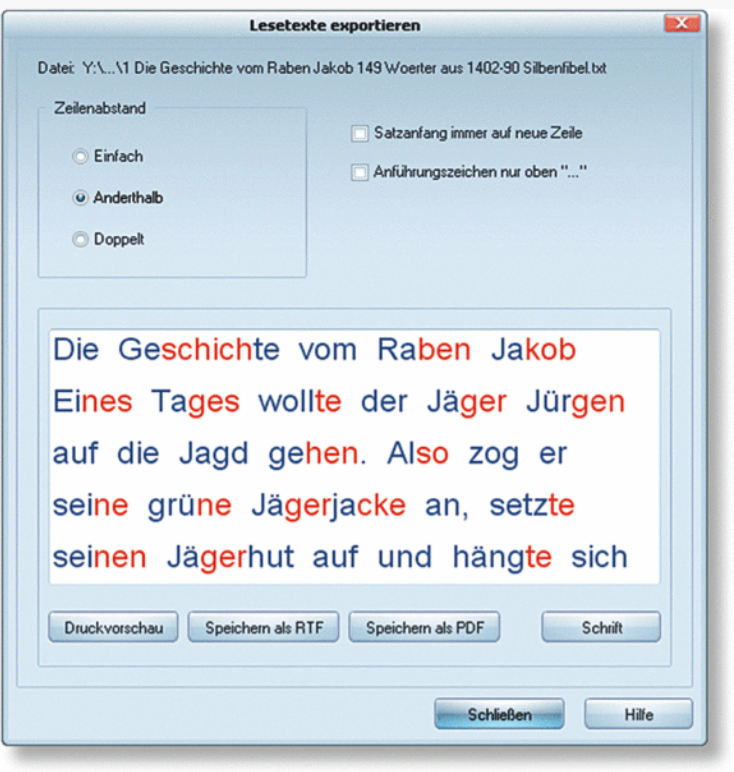
\includegraphics[width=.5\linewidth]{figures/ABCsilbengenerator}
	\caption{Bildschirmfoto des Silbengenerators auf der Internetseite von \textit{ABC der Tiere}\cite{ABCSilbengenerator2018}}
	\label{fig:ABCsilbengenerator}
\end{figure}
Ein weiteres zu erwähnendes Tool ist die \textit{Celeco Druckstation}\cite{celeco2018}. Auch hier können eigene Texte entweder mit farblich markierten Silben oder Silbenbögen gedruckt werden. Das Programm ist zusammen mit der \textit{Celeco} Software (LRS Therapie und Leseübungen) erhältlich, welche für Windows verfügbar ist.

Um die Vorteile durch silben- und betonungsorientiertes Lernen auszunutzen ist man oft auf Materialien von Verlagen oder eine aufwendige manuelle Erstellung von Texten angewiesen. Dies bekräftigt die Motivation eine neue Lösung zu entwickeln um eigenes Übungsmaterial erstellen zu können, was zudem flexibel gestaltbar und z.B. auf bestimmte Schüler anpassbar ist.

\section{Technischer Hintergrund}

Um das Ziel einer automatischen Analyse und Annotation beliebiger Texte zu realisieren, wurden vor Allem die folgenden zwei Schritte untersucht:
\begin{enumerate}
	\item Linguistische Analyse (Zerlegung des Texts in Wörter)
	\item Bestimmung von Silbentrennung und Betonungsmuster
\end{enumerate}

\subsection{Linguistische Analyse}
Da die von der Applikation zu verarbeitende Eingabe ein Text ist, also eine beliebige Folge von alphanumerischen Zeichen, sowie Leerraumzeichen und Interpunktionen, muss diese Eingabe zunächst korrekt in Wörter zerteilt werden. Dieser Schritt wird \textbf{Tokenisierung} genannt. Zusätzlich werden auch von einem \textbf{Tagger} jedem Wort weitere Informationen, wie z.B. die Wortart (\textit{Part-of-Speech-/POS-Tagger}) hinzugefügt. Diese werden üblicherweise mithilfe eines entsprechenden Lexikons nachgeschlagen\cite{Carstensen2004}. Der für dieses Projekt verwendete Parser wird in Abschnitt \ref{sec:spacy} näher beschrieben. Beim Parsen des Texts können folgende wichtige Informationen extrahiert werden:

\begin{itemize}
	\item \textbf{Textstruktur}: Zerlegung des Texts in Tokens, dadurch wird bestimmt, ob es sich bei den Zeichenfolgen um Wörter oder andere Strukturen wie Leerraum oder Interpunktionen handelt.
	
	\item \textbf{Wortart}: Die Werte der Wortart- (\textit{Part-of-Speech-}) Tags geben an um was für ein Wort es sich handelt (mit dem \textit{spacy} Parser z.B. \textit{NOM} für Nomen, \textit{PROPN} für Eigennamen, \textit{DET} für Artikel etc.).
	\item  \textbf{Lemma}: Gibt die Grundform eines Wortes an, welche je nach Wortart unterschiedliche Ausprägungen annehmen kann. Bei Verben steht hier z.B. der Infinitiv, bei Pronomen die erste Person Singular etc.
\end{itemize}

\subsection{Datenbank zur Wortbetonung}
\label{sec:forschung-database}

Liegt der Text als Liste von Wörtern (Tokens) vor, so können weitere Analysen auf dieser Ebene vorgenommen werden. Für die Annotation des Textes muss eine Repräsentation in Silben vorliegen, zusätzlich wird die betonte Silbe im Wort gesucht. Es ist durchaus möglich, dass in einem Wort mehrere Betonungen vorkommen (gerade bei Wortkompositionen, die im Deutschen häufig zu finden sind, z.B. \textit{heraus+kommen}). Dies wird hier vernachlässigt, es wird nur eine Hauptbetonung, die erste vorkommende Betonung im Wort gesucht. Eine weitere Einschränkung die getroffen wurde ist die Beschränkung auf die Annotation der Betonung im Wort-Kontext (und nicht im Zusammenhang des Satzes). Hier wäre es auch denkbar gewesen, für die Erlernung von Sprachrhythmus und Satzmelodie die Betonung über Wortgrenzen hinaus in Sätzen hervorzuheben. Folgen z.B. viele kurze Wörter aufeinander, so werden diese im natürlichen Sprachrhythmus nicht alle gleich betont gesprochen, sondern eine Betonung findet nur in bestimmten Wörtern im Satz statt. Im Rahmen der vorliegenden Arbeit wurde dieser Aspekt der Prosodie vernachlässigt. Das Ziel war es, bei Menschen mit LRS die Dekodierung des Wortbildes mithilfe von Silben zu erleichtern, daher wurde sich auf die Möglichkeit konzentriert, einzelne Silben und die betonte Silbe im Wort hervorzuheben.\\

Informationen zur Worttrennung in Silben und zur Wortbetonung lassen sich in diversen Lexika finden. \todo{Welche: PhonoLex Core mit Balloon, generell Wörterbücher für Silbentrennung, Hyphenator von OpenOffice oder LaTex} Für die weitere Verwendung in der zu entwickelnden Applikation wurde als Grundlage das Lexikon CELEX2 gewählt. Dabei handelt es sich um ein umfangreiches Sprachlexikon für die Sprachen Englisch, Deutsch und Niederländisch. Verarbeitet wurden hier zunächst nur die deutsche Sprache. Neben der gesuchten Worttrennung und -betonung enthält es auch weitere linguistische Informationen wie Wortart und Grundformen, sowie phonologische und orthographische Annotationen \cite{Burnage1990}. \todo{Alternativen, welche? könnten zusätzlich oder anstelle des CELEX verwendet werden. z.b. PhonoLex Core, besser als CELEX, umfangreicher (quelle!), aber nicht kostenfrei}

Weiterführend wurden auch Text-To-Speech Systeme untersucht. Diese generieren bei gegebenem Eingabetext automatisch synthetische Sprache. Dazu wird intern ein phonologisches Modell aufgebaut, um zu funktionieren muss also zwangsweise eine phonologische Analyse durchgeführt werden, welche auch die Wortbetonung bestimmt. Beispielsweise liefern die Systeme MARY TTS\tocite{MARY} oder BAS\tocite{BAS} auch textuell annotierte Formen ihrer phonologischen Analyse, die als Grundlage zur Extraktion von Betonung dienen können.\\

Linguistische Datenbanken können aufgrund des Umfangs und der Flexibilität von Sprachgrammatiken niemals vollständig sein. Es wurde daher ein Weg gesucht die Datenbank auf unkomplizierte Weise erweiterbar zu machen. Dies kann mit einem geeignete User-Interface durch ExpertInnen erfolgen, die unbekannte Einträge ergänzen und hinzufügen. Einige Arbeiten hatten bereits Erfolg damit, solche Aufgaben durch \textit{Croudsourcing} effektiv auch auf Nutzer zu verteilen, die keine ExpertInnen für den jeweiligen Anwendungsbereich sind. Da die zu entwickelte Applikation auch ein Nutzerverwaltungssystem beinhaltet, wurde untersucht, ob Datenbankeinträge mithilfe mehrerer Nicht-Experten NutzerInnen per einfachem Mehrheitsentscheid verifiziert werden können. Weiterführend könnten auf Plattformen wie Amazon Mechanical Turc oder CrowdFlower beispielsweise leicht Arbeiter anonym engagiert werden, die solche Aufgaben erledigen\cite{Snow2008}. Diese Plattformen wurden beispielsweise von Zaidan und Callison-Burch (für automatisierte Übersetzungen)\cite{Zaidan2011} oder De Kuthy, Ziai und Meurers\cite{Meurers2015} (für Fokusannotation) benutzt, um computerlinguistische Aufgaben zu erledigen.
\cleardoublepage

% !TEX root = ../ausarbeitung.tex

\chapter{Anforderungsanalyse und Spezifikation}

Schon während der Konzeption des Projekts ist klar geworden, dass die zu entwickelnde Software eine relativ komplexe Architektur erfordert. Da eine Browser Applikation entwickelt wurde, musste die Software in Teilprojekte untergliedert werden. Zum einen das User-Interface für die Web Applikation und zum Anderen die Programmlogik, welche auf Grund der benötigten Funktionalitäten (wie Datenbankanbindung und Algorithmen zur Textverarbeitung) nicht sinnvoll im Web Client implementiert werden konnte.\\
Um eine Spezifikation für die Software zu entwerfen und den zu verwendenden Software-Stack zu definieren, wurde zunächst eine Anforderungsanalyse durchgeführt, die im Folgendem Teil beschrieben wird. Im darauffolgenden Kapitel gehe ich Schritt für Schritt auf die Entwicklung des Gesamtsystems ein.

\section{Anforderungen an die Software}

Zunächst wurde festgestellt, welche Funktionen die App dem Nutzer bieten soll. Dazu wurden Folgende mögliche Szenarien aufgestellt:

\paragraph{Text Analyse} 
Der User möchte einen Fließtext eingeben und von der Anwendung annotieren lassen. Nach der Eingabe soll das Ergebnis annotiert in der App dargestellt werden.

\paragraph{Anpassung der annotierten Darstellung}
Der User möchte die Parameter des annotierten Texts ändern. Angepasst werden können sollen die Texteigenschaften (Font, Zeilenabstand, Zeichenabstand) und die Darstellung der Annotation (Farben für betonte und unbetonte Silbe, Silbenabstand, Trennzeichen zwischen Silben)

\paragraph{Export der annotierten Darstellung}
Der User hat die Möglichkeit verschiedene Formate des annotierten Texts zu exportieren, z.B. Druck, HTML oder Word.

\paragraph{Verwaltung von User Accounts}
Dem User soll die Möglichkeit gegeben werden, einen User Account zu erstellen um persönlich verwendete Daten (z.B. Texte oder Wortsegmentierungen) speichern zu können. Dazu werden Funktionen und Interfaces zur Registrierung eines Nutzeraccounts, Login, Logout, zum Bearbeiten der Nutzerinformationen und zum Löschen des Accounts bereitgestellt.

\paragraph{Behandlung unbekannter Wörter}
Der Nutzer kann nacheinander die Segmentierung von Wörtern, die durch das System nicht eindeutig bestimmt wurden konnten, selbst manuell festlegen.

\paragraph{Bestimmung der Segmentierung unbekannter Wörter}
Für ein unbekanntes Wort wählt der User in einem neuen View die Segmentierung selbst aus. Dafür werden folgende Möglichkeiten gegeben:
\begin{itemize}
	\item Input aus G2P Systemen wie MARY TTS
	\item Manuelle Segmentierung mit geeignetem User Interface
	\item Eventuell weitere Quellen für die Segmentierung (z.B. Duden)
\end{itemize}

\paragraph{Speicherung von Nutzer Segmentierungen}
Vom Nutzer hinzugefügte Segmentierungen sollen (lokal für diesen Nutzer) gespeichert werden können und beim nächsten Vorkommen in einem Text automatisch verwendet werden.

\paragraph{Speicherung und Wiederverwendung von Annotationskonfigurationen für Texte}
Die Einstellungen, die ein Nutzer an einenm annotierten Text vorgenommen hat, können als Vorlage für andere Texte gespeichert werden. In den Annotationseinstellungen eines Textes kann eine zuvor gespeicherte Konfiguration wiederverwendet werden.

\paragraph{Speicherung und Wiederverwendung von Nutzertexten}
Analysierte Texte können vom Nutzer zusammen mit der verwendeten Konfiguration gespeichert werden. Den Texten können Metadaten zugeordnet werden, z.B. Thema, Niveau, Zielgruppe. Im Benutzerbereich werden die Texte, die der Nutzer hinzugefügt hat, geeignet strukturiert, dargestellt. Dem Nutzer wird die Möglichkeit gegeben, den gespeicherten Text erneut analysieren zu lassen.

\paragraph{Verifizierung unbekannter Wörter}
Manuelle Segmentierungen von unbekannten Wörtern müssen auf Korrektheit überprüft werden. Dazu wird jeder Nutzer aufgefordert, die Einträge anderer Nutzer zu überprüfen. In einem View, ähnlich zur manuellen Segmentierung, kann der Nutzer Einträge anderer Nutzer bestätigen oder Gegenvorschläge übermitteln.

\paragraph{Expertennutzer}
Ein Experte (z.B. Linguist oder Lerntherapeut) kann sich als solcher bei der Erstellung eines Accounts identifizieren. Bei der Wort Verifizierung zählt die Stimme der Expertennutzers mehr als die eines Nutzers, der kein Experte ist.

\subsubsection{User Interface}
Von diesen Szenarien ausgehend wurde in den Folgenden Schritten ein geeignetes User Interface erarbeitet:

\paragraph{Informationsstruktur}
\todo{information structure, menü hierarchie, aufbau des user interfaces (links, lineare hierarchie), storyboards}\\

\paragraph{Farbschema}
\todo{color scheme https://color.adobe.com}

\subsection*{Grundlegende Anforderungen}

Aus den oben beschriebenen Use Cases lassen sich diverse Anforderungen an die Software spezifizieren:

\begin{itemize}
	\item Service zur Textanalyse
	\item Wortdatenbank
	\item Service zur Manipulation der Wortdatenbank
	\item Service zur Nutzerverwaltung
	\item Speicherung Nutzer spezifischer Daten
	\item Geeignetes User Interface zur Darstellung von Texten und zur Interaktion mit dem System
\end{itemize}




\section{Softwarestack}

Bei der Vielseitigkeit der verschiedenen Anforderungen ist die Wahl der zu verwendenden Technologien nicht unerheblich. Programmiersprachen und Frameworks müssen sorgfältig ausgewählt werden um für jedes Teilproblem eine passende Lösung zu entwickeln.\\
Die erste wichtige Unterteilung fand statt zum Einen in ein Frontend welches die zum Benutzer darstellt und zum Anderen in ein Backend welches die vom System verwendeten Daten speichert und manipuliert und diese mit Hilfe geeigneter Algorithmen an das Frontend schickt. Eine genaue Beschreibung über den detaillierten Aufbau und die Funktion von Front- und Backend wird in Kapitel 4 gegeben.\\

\todo{kleine Grafik zu front backend}

Diese Aufteilung ist in der Webentwicklung weit verbreitet \tocite{front backend} und bietet einige Vorteile gegenüber eins komplett integriertem Gesamtsystems:

\begin{itemize}
	\item Klare Trennung von Darstellung und Datenverarbeitung
	\item Einfachere Fehlersuche durch kleinere Komponenten
	\item Bei der Entwickelung zusätzlicher Frontends (z.B. für Android oder iOS) muss nur ein neuer Teil des Softwaresystems entwickelt werden, während das Backend gleich bleibt
	\item Einfache Arbeitsaufteilung im Entwicklerteam (relevant bei Weiterentwicklung der Anwendung mit mehreren Personen)
	\item \todo{more?}
\end{itemize}

\subsection{Verwendete Technologien}
Für verschiedene zu realisierende Ziele gibt es für jedes Teilziel Technologien, die Vorteile gegenüber anderen bieten. Die Verwaltung von Datenbanken ist zum Beispiel besser mit einer Server seitigen Skriptsprache zu implementieren, als mit den Möglichkeiten, die das Frontend bietet. Im Web Frontend dagegen sind gewisse Technologien wie HTML, CSS und JavaScript standard, die zwangsläufig verwendet werden müssen. Daher wird In der Applikation eine Vielzahl verschiedener Technologien verwendet, eine Übersicht ist hier gegeben:

\begin{itemize}
	\item Backend: python, REST API, sowie die python Frameworks flask, spacy und sqlalchemy
	\item Frontend: HTML, CSS, JavaScript, AngularDart
	\item Kommunikation mit JSON
	\item Deployment mit Apache auf AWS Server
\end{itemize}

Im Folgenden werden die einzelnen Technologien und deren Vorteile beschrieben.

\subsection{Backend}
Backend as a service: e.g. Firebase, zu unflexibel\\

welche alternativen fuer backend\\
frontend unabhäng von daten

\subsubsection{python}
warum python\\
flexibel und schnell, viele frameworks\\
Requests an externe Services, MARY, BALLOON

\subsubsection{REST API}
was? warum?

\subsubsection{flask}
gutes framework für REST

\subsubsection{spacy}
parser, alternative NLTK, auch benutzt, warum ist spacy besser?\\
tokenizer, part of speech

\subsection{Frontend}

webapplication, html css, single-view-application, dynamic data loading
viele frameworks, verwende AngularDart
no javascript: weakly typed languages transforming to JS: GWT (java), typescript, Dart

\subsubsection{Angular Dart}
warum? javascript is bad.\\

data binding\\
more lightweight vs Java\\

many google apps use it\\
objektorientierung\\

angular? angular2?\\

dart, google\\
alternativen, typescript...\\

dart2js compiler, wie funktioniert dieser\\

\subsection{Deployment}

webserver für frontend, auf eigenem server mit apache gehostet\\
flask python service läuft immer, REST schnittstelle\\






%-----------------------------------------------------------------------------------------
%-----------------------------------------------------------------------------------------

\cleardoublepage

% !TEX root = ../ausarbeitung.tex

\chapter{Evaluation}

Die Applikation wurde mit dem Hauptziel entwickelt, eine Nutzeroberfläche zu entwickeln, mit der sowohl Personen, die in der LRS Therapie arbeiten (wie Lerntherapeuten oder Nachhilfelehrer) als auch Nicht-Experten (z.B. die Eltern betroffener Kinder) intuitiv und effizient benötigtes Arbeitsmaterial erstellen können. Außerdem wurde untersucht wie eine Datenbank für Betonungsmuster in Wörtern erstellt und benutzerfreundlich erweitert werden kann.\\

Die Evaluation untersucht daher folgende Punkte:
\begin{itemize}
	\item Erstellung von Arbeitsmaterial aus einem einfachen Text 
	\item Intuitivität und Einfachheit der Bedienung
	\item Effizienz des Prozesses der Erstellung von Arbeitsmaterial
	\item Unterschiede in der Bedienung durch Experten und Laien
	\item Nutzerfreundliche Erweiterung der Wortdatenbank
\end{itemize}

Zunächst wird durch Beispiele eines annotieren Textes mit verschiedenen Einstellungen demonstriert, welche vielseitigen Möglichkeiten die Textannotation für das Erstellen von Arbeitsmaterial bietet. Für die Untersuchung von Intuitivität, Einfachheit und Effizienz bei der Bedienung der Applikation wurde ein Nutzertest durchgeführt. Dieser fand als Interview statt um qualitative Daten durch Nutzerbefragung zu erheben. Außerdem wurden quantitative Daten durch das Ausfüllen von Ankreuzfragen während des Interview erhoben.

\section{Ergebnisse der Textannotation}

Um zu zeigen, dass die Applikation das Ziel des automatischen Erstellens von Arbeitsmaterial erfüllt, werden im Folgenden verschiedene Texte präsentiert, die mit Hilfe des Web Interfaces erstellt wurden. Die Ergebnisse zeigen, dass das Programm diese Ziel nicht nur erfüllt, sondern im Vergleich zu herkömmlichen Methoden \tocite{Silbefibel, ABC} auch noch einen hohen Grad an Flexibilität bietet. Die Einstellungen und damit das Erscheinungsbild des resultierenden Textes können vom Nutzer frei an die Bedürfnisse des jeweiligen Falls angepasst werden.\\

Im Folgenden wurde der Beispieltext \textit{Aschenputtel} mit der Web Applikation analysiert, sodass Silbentrennung und Betonung farblich markiert dargestellt werden. Die in den Beispielen verwendeten Texten wurden mit der Druckfunktion der Textvorschau als PDF Dateien exportiert. Jedes Bild entspricht einer DIN A4 Seite.

\subsubsection{Beispiel 1: Hervorhebung der Silben mit zwei alterierenden Farben}

Im ersten Beispiel wird die Schriftfarbe für da Hervorheben der Silben genutzt. Die betonte Silbe wird immer rot dargestellt, in Wörtern mit vielen Silben, werden diese dann alterierend rot und blau hervorgehoben. Die Schriftgröße wurde auf \textit{22} gesetzt, der Wortabstand auf den Wert \textit{0.4}. Zusätzlich sorgt die Einstellung des Zeilenabstands auf \textit{1.5} für bessere Lesbarkeit.

\begin{figure}[h!]
	\centering
	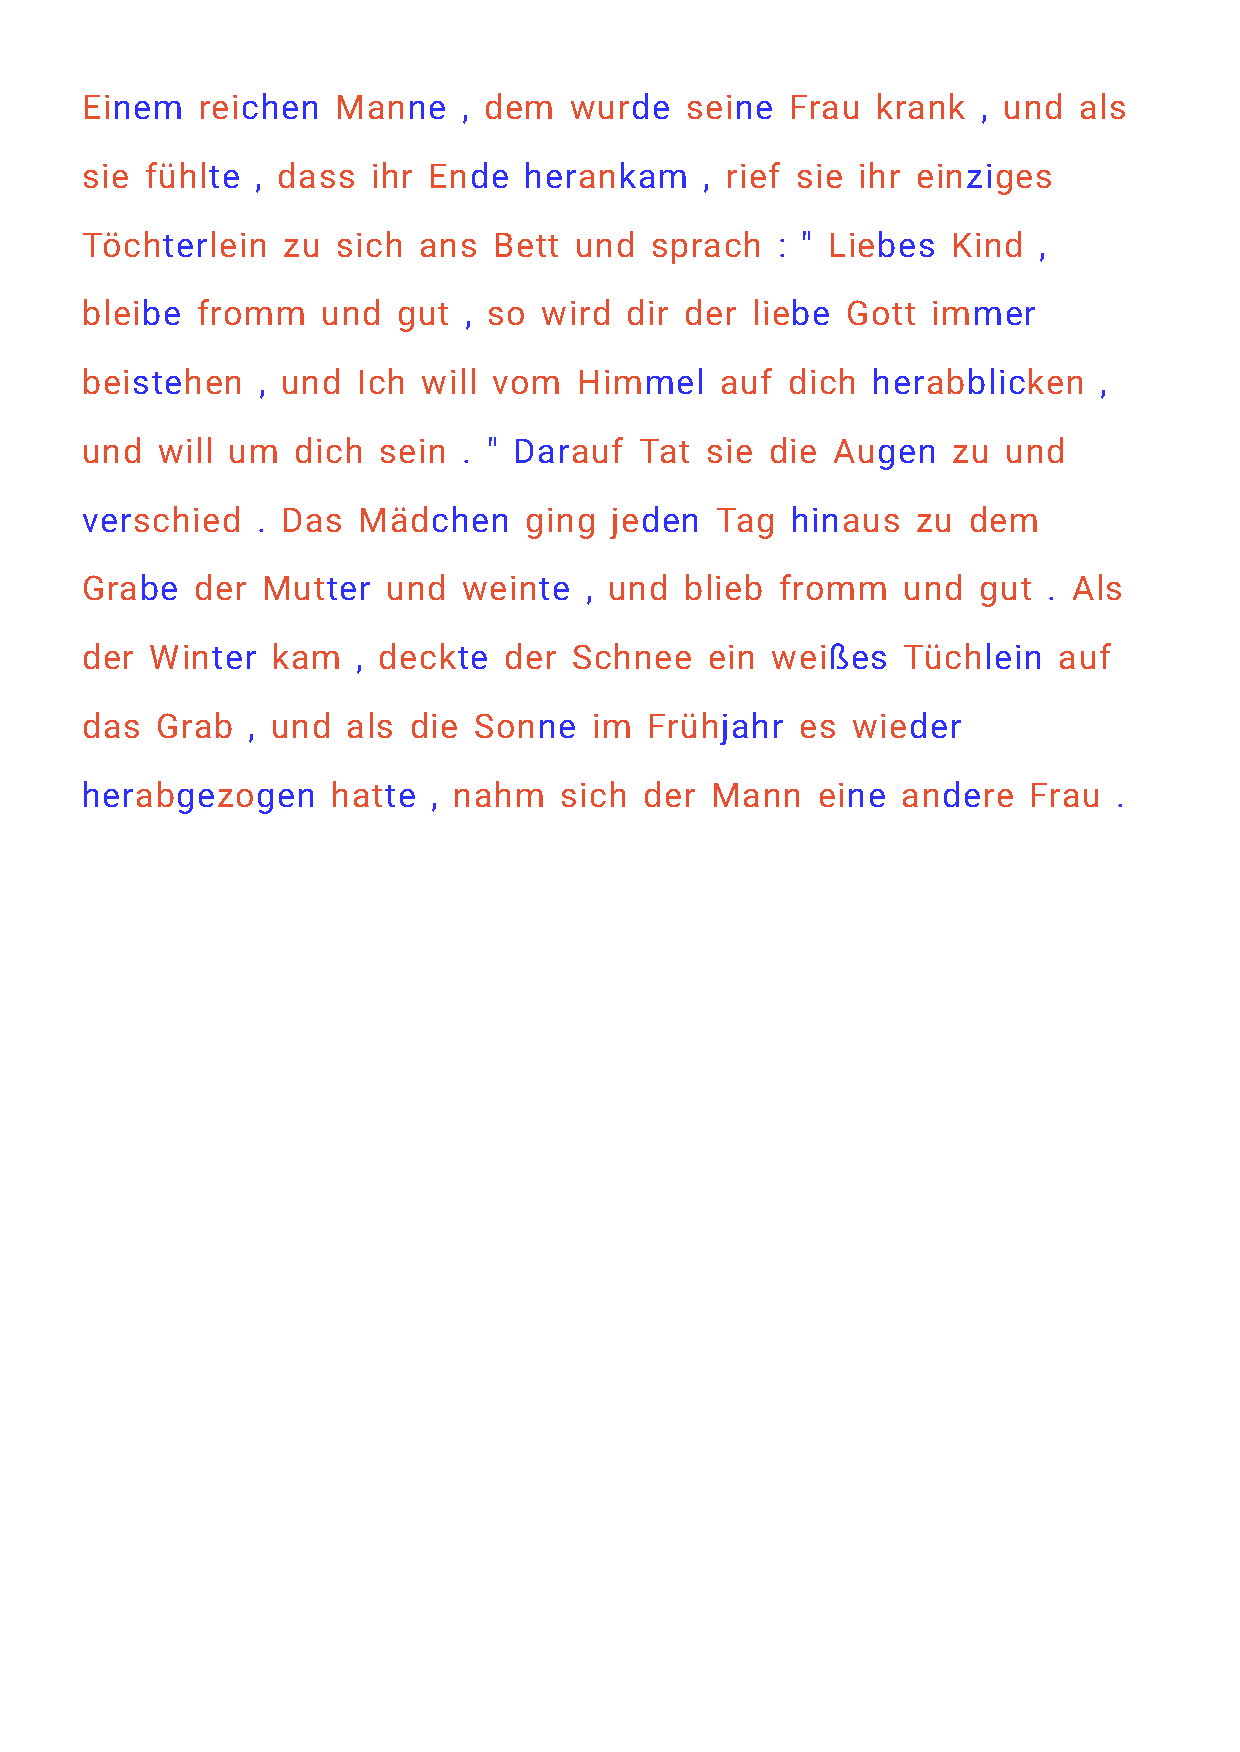
\includegraphics[width=.7\linewidth, frame]{figures/evaluation/annotation1}
	\caption{Hervorhebung der Silben mit zwei alterierenden Farben}
	\label{fig:evaluation-ex1}
\end{figure}
\newpage

\subsubsection{Beispiel 2: Worthintergrund und Silbenabstand}

In diesem Beispiel sorgt die Worthintergrundfarbe für eine bessere Wahrnehmung des Wortes als Einheit. Dadurch kann auch ein Silbenabstand (hier \textit{0.1}) eingestellt werden ohne dass die Gefahr besteht, dass dadurch nicht mehr klar ist, welche Silben zusammen gehören. Wegen dem Worthintergrund nehmen die Wörter mehr Platz in der Zeile ein, daher wurde auch der Zeilenabstand auf \textit{2.2} erhöht. Zudem wurde hier ein Zeichenabstand von \textit{2} (statt \textit{1} in Beispiel 1) gewählt.

\begin{figure}[h!]
	\centering
	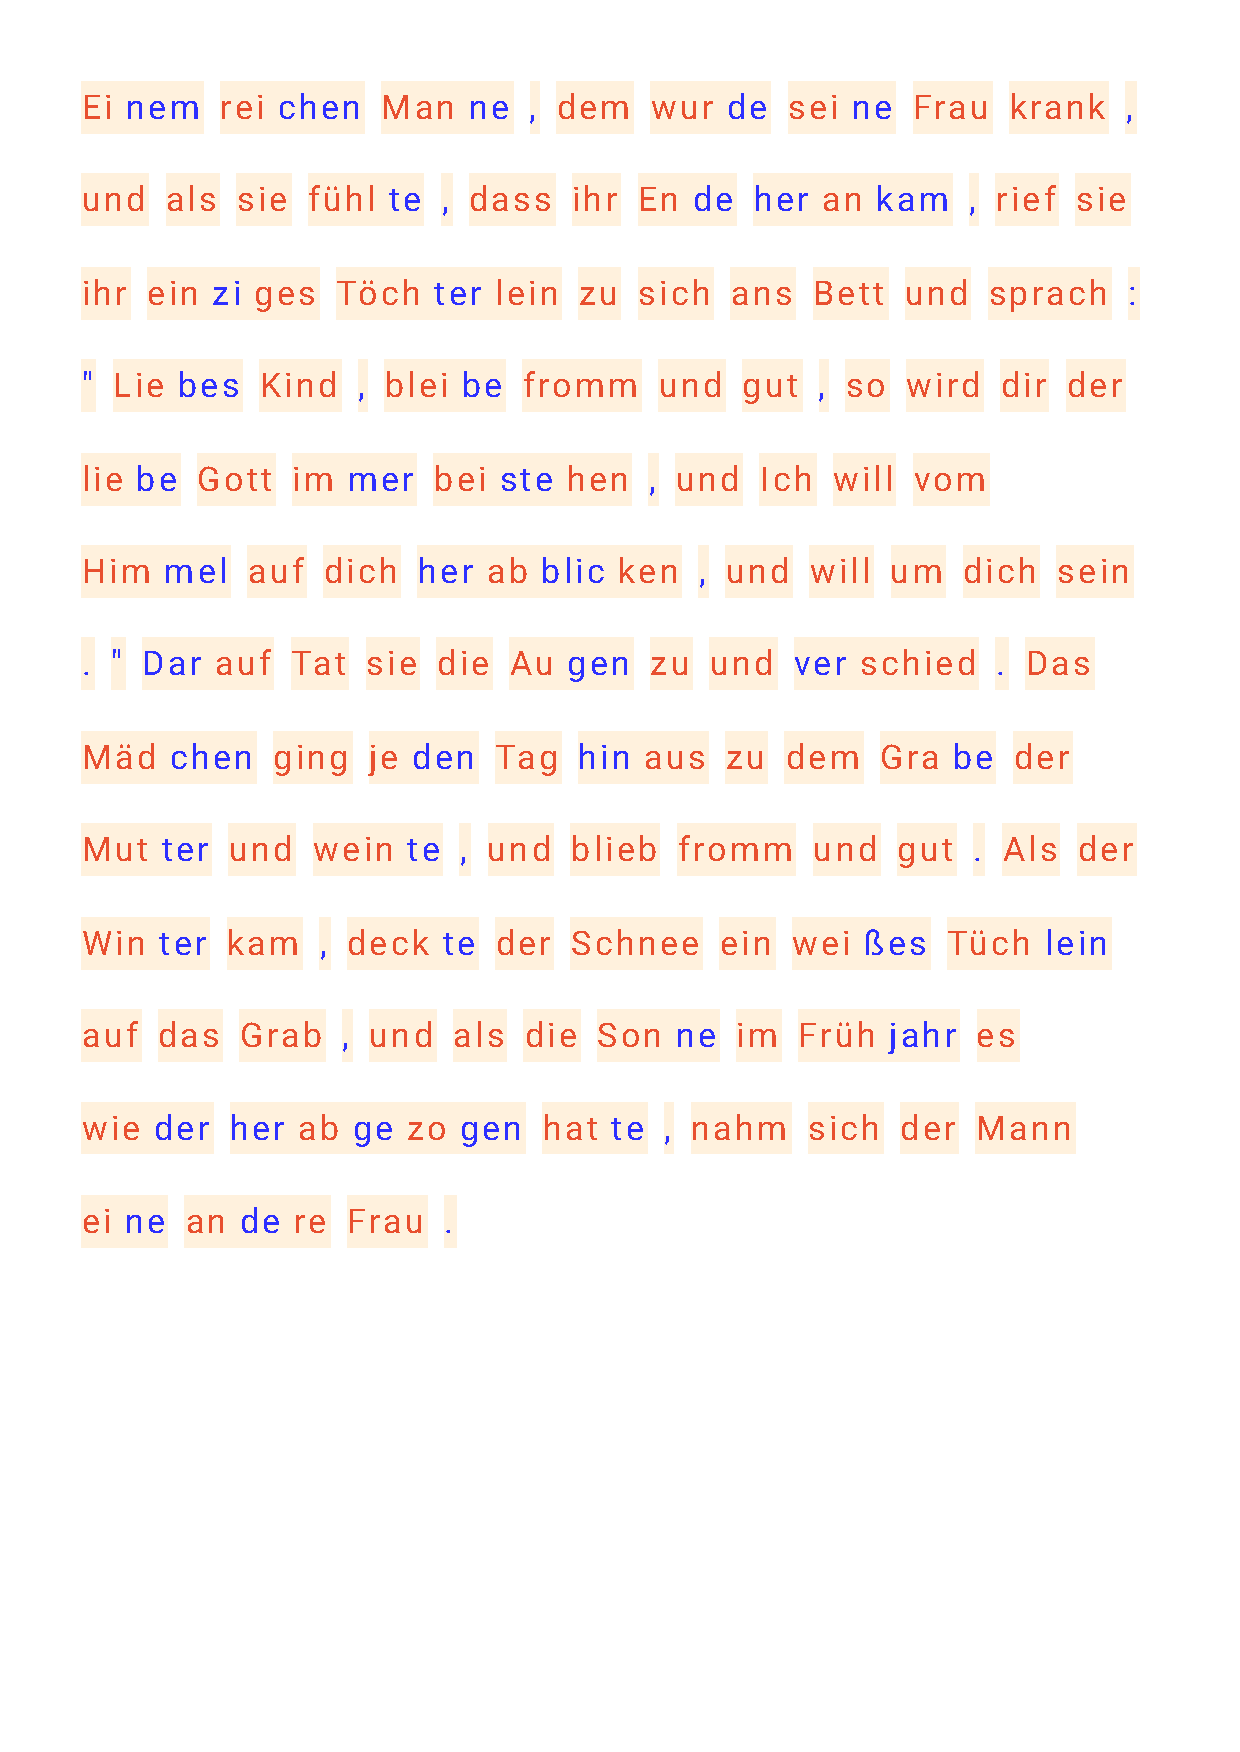
\includegraphics[width=.7\linewidth, frame]{figures/evaluation/annotation2}
	\caption{Worthintergrund und Silbenabstand}
	\label{fig:evaluation-ex2}
\end{figure}
\newpage

\subsubsection{Beispiel 3:  Silbentrennzeichen und verschiedene Silbenfarben}

In Beispiel 3 wurde wieder auf die Worthintergrundfarbe verzichtet. Das Trennzeichen \qq{=} soll hier das Silbentrennen erleichtern, sowie zusammenhängende Silben zu einem Wort gruppieren. Der Zeichenabstand beträgt wieder \textit{1}, der Silbenabstand \textit{0}, da das Gleichheitszeichen hier als Silbentrenner dient. Zusätzlich wurde eine weitere Farbe für alterierende Silben gewählt. Hier wird nur noch die betonte Silbe rot dargestellt, danach alterieren die Silben bei langen Wörtern in den Farben blau und lila.

\begin{figure}[h!]
	\centering
	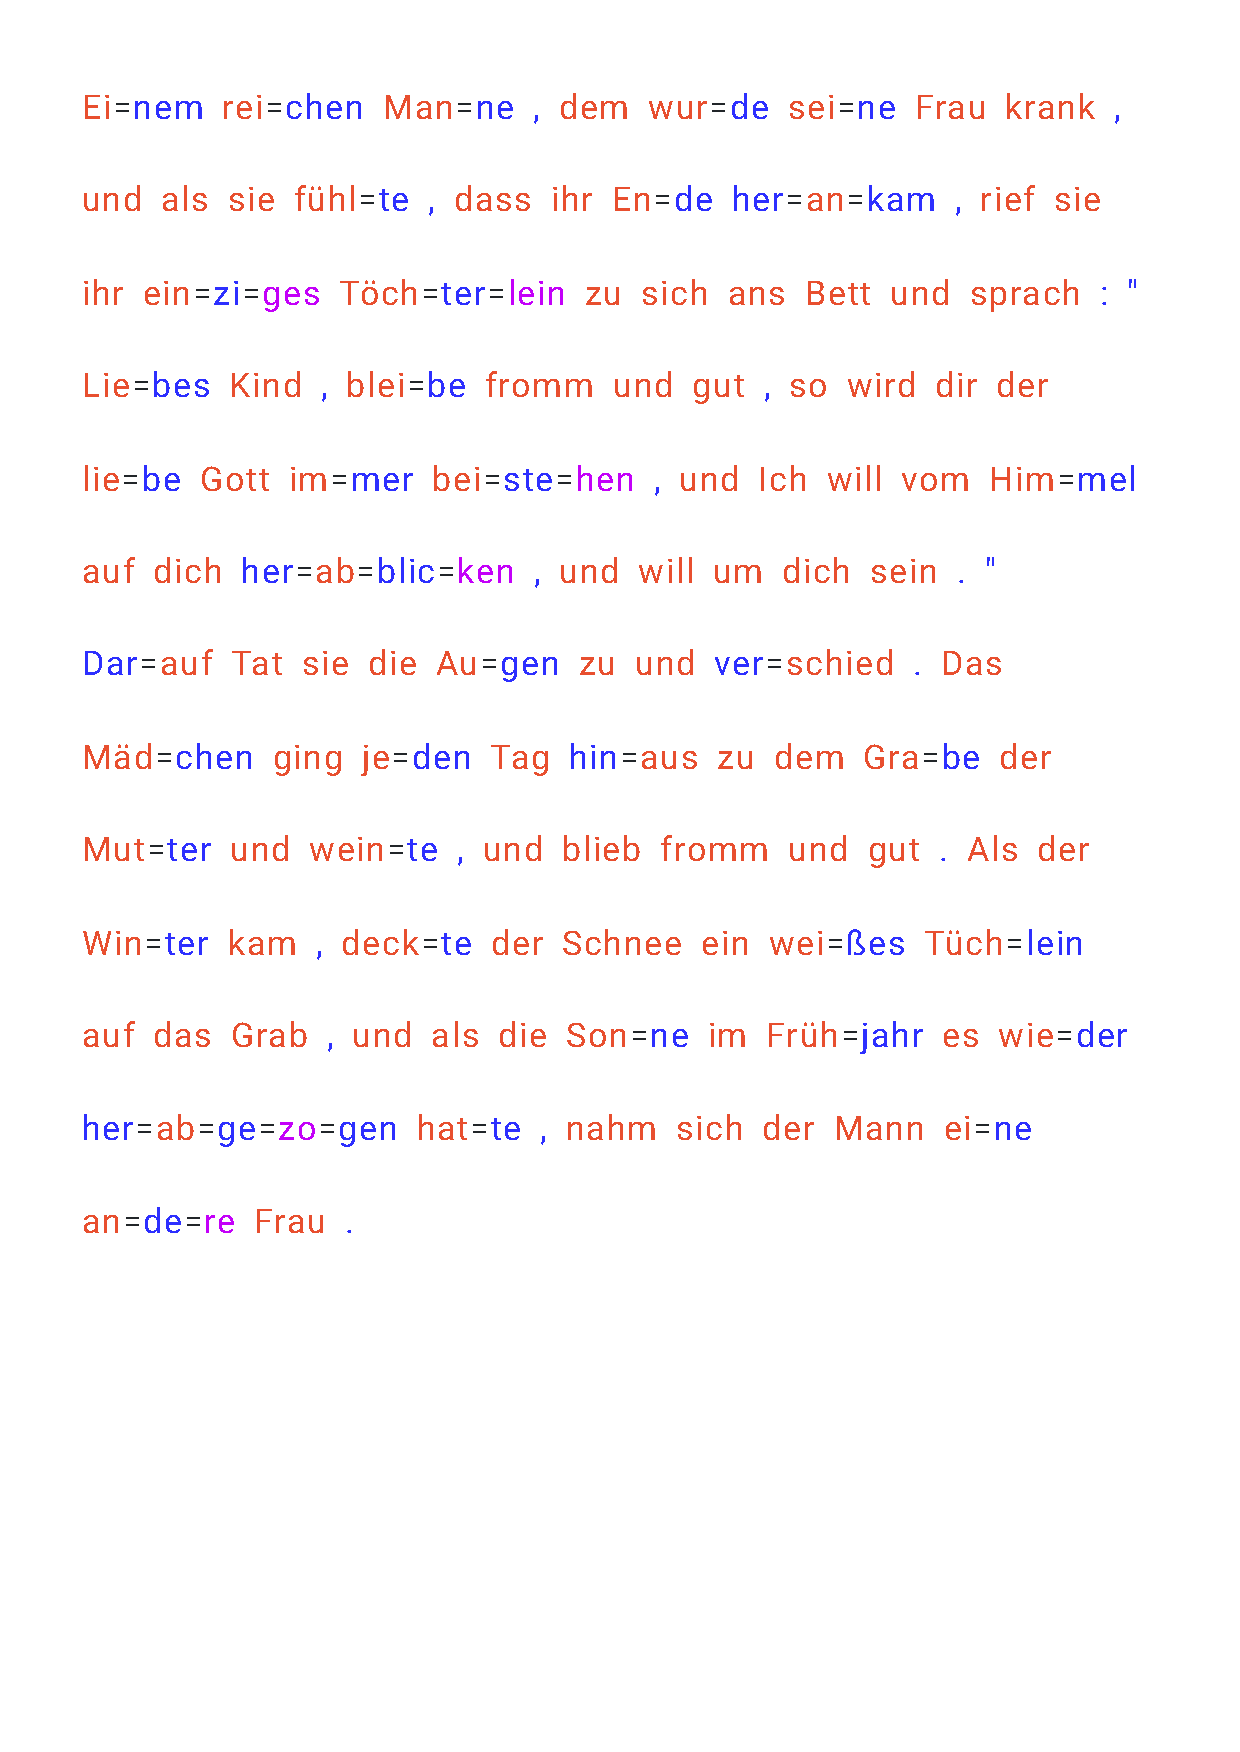
\includegraphics[width=.7\linewidth, frame]{figures/evaluation/annotation3}
	\caption{Silbentrennzeichen und verschiedene Silbenfarben}
	\label{fig:evaluation-ex3}
\end{figure}
\newpage

\subsubsection{Beispiel 4: Hervorhebung des Silbenhintergrunds}

In diesem Beispiel wird ein anderer Ansatz der farblichen Hervorhebung gewählt. Die eingestellten Farben bestimmen hier den Hintergrund der Silben und nicht die Schriftfarbe (diese ist immer Schwarz). Das Beispiel hebt vor Allem die betonte Silbe hervor, die grün dargestellt werden. Unbetonte Silben bekommen alterierend zwei verschiedene Grautöne als Hintergrund. Der Silbenabstand ist hier wieder \textit{0}, somit wird die Einheit des Wortes deutlich erkennbar.

\begin{figure}[h!]
	\centering
	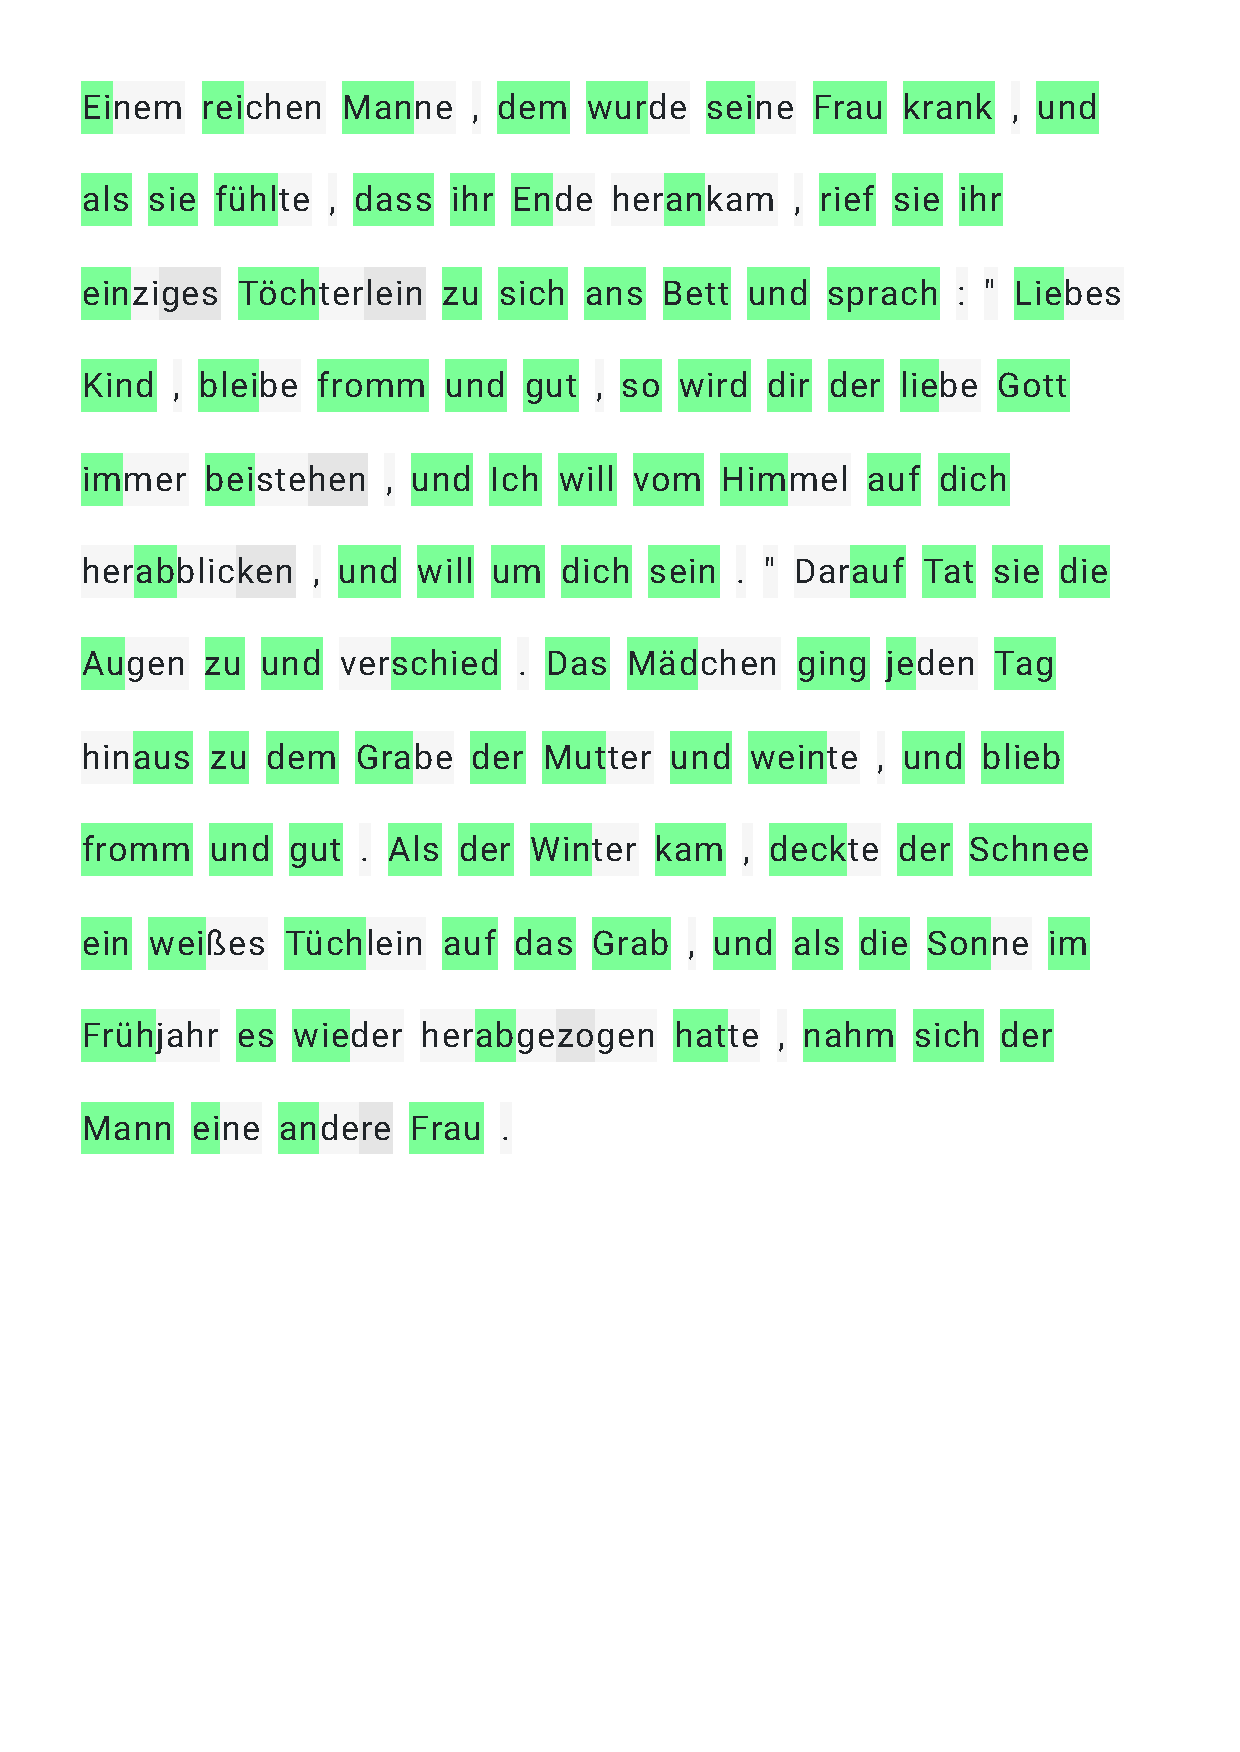
\includegraphics[width=.7\linewidth, frame]{figures/evaluation/annotation4}
	\caption{Hervorhebung des Silbenhintergrunds}
	\label{fig:evaluation-ex4}
\end{figure}
\newpage

\subsubsection{Beispiel 5: Manuelles Deaktivieren der Hervorhebung in kurzen Wörtern}

In Beispiel 5 wird der Sprachrhythmus mit Wortbetonungen noch deutlicher hervorgehoben. Die betonte Silbe wir zusätzlich zur grünen Farbe auch fett dargestellt. Außerdem wurde die Betonung in manchen Wörtern deaktiviert, so werden im ganzen Text beispielsweise Artikel, Präpositionen oder manche einsilbigen Wörter nicht betont markiert. Dieser Text soll damit einen Fokus auf den Sprachrhythmus innerhalb ganzer Sätze legen.

\begin{figure}[h!]
	\centering
	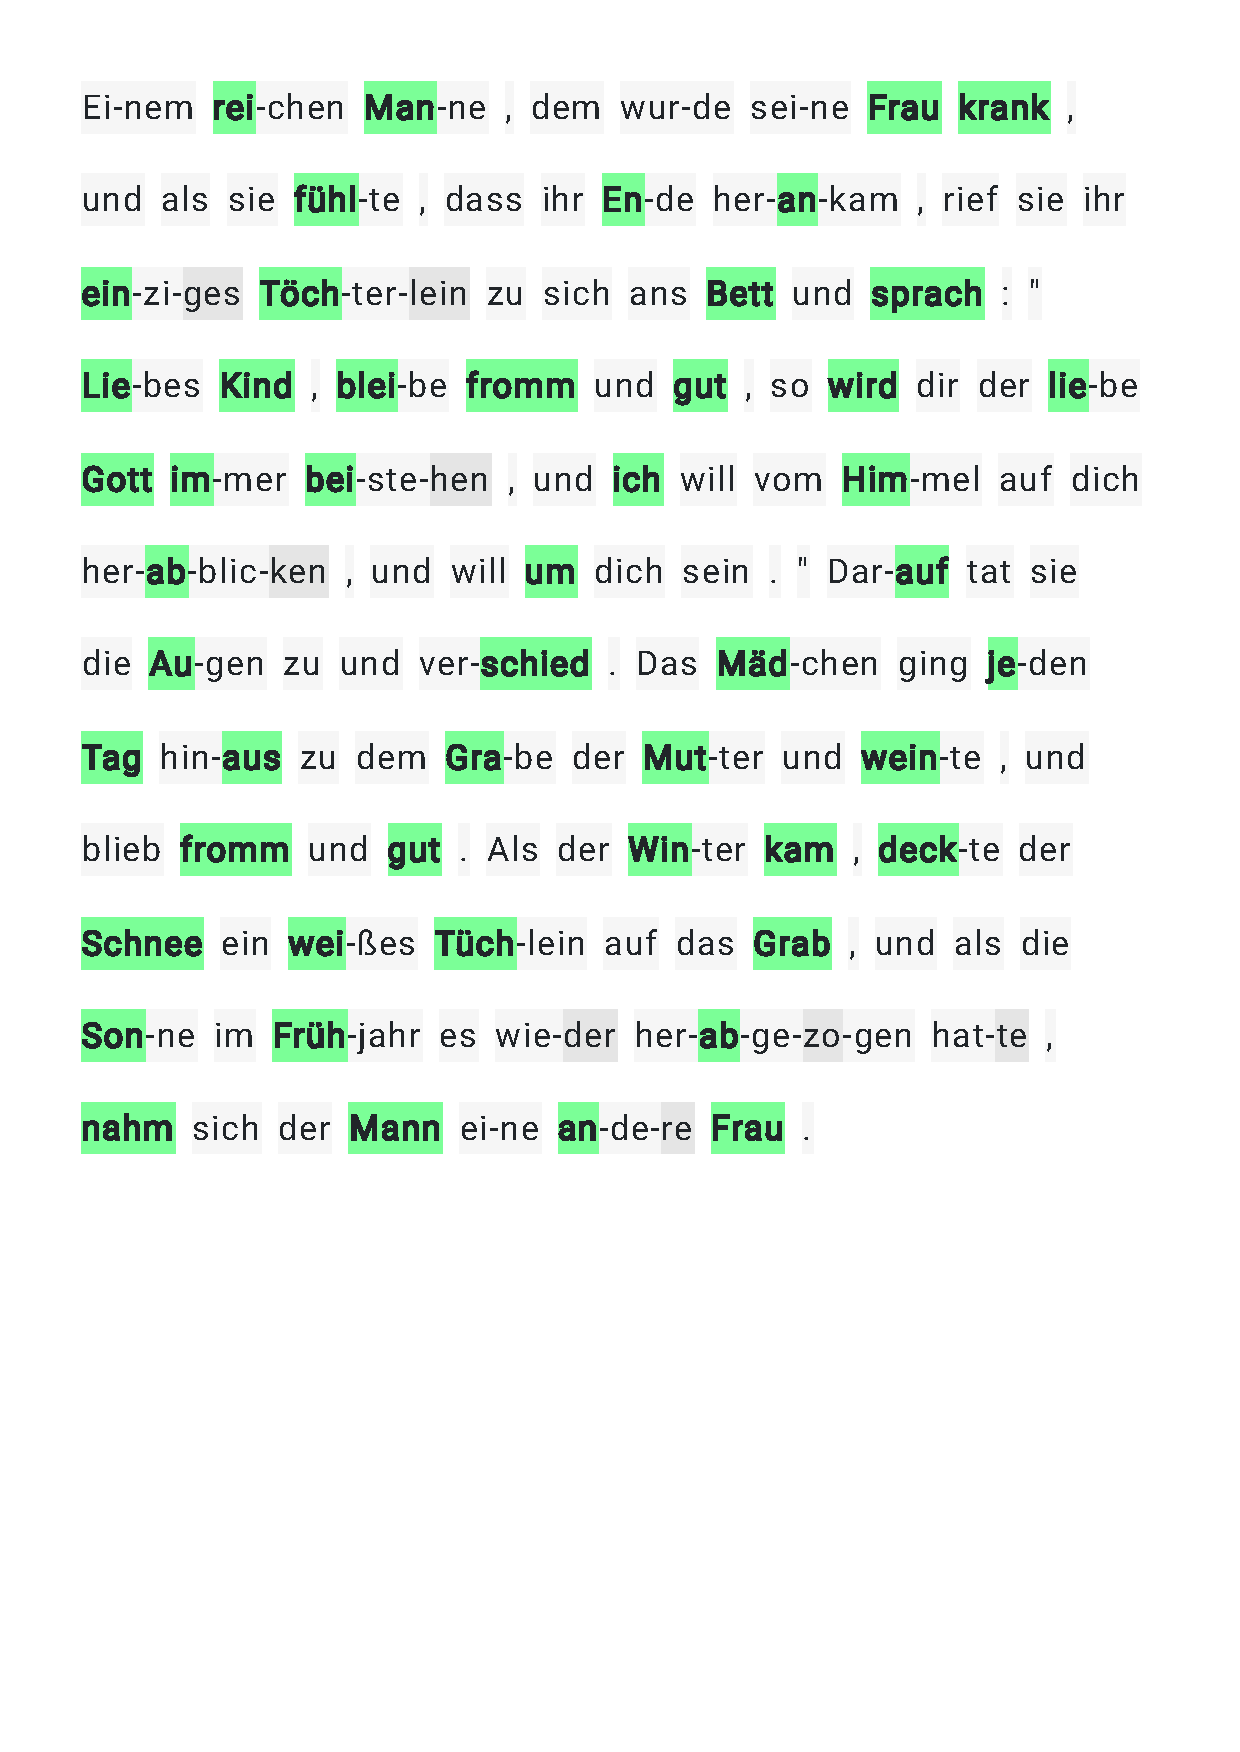
\includegraphics[width=.7\linewidth, frame]{figures/evaluation/annotation5}
	\caption{Manuelles Deaktivieren der Hervorhebung in kurzen Wörtern}
	\label{fig:evaluation-ex5}
\end{figure}
\newpage

\section{Nutzertest}

Während die Beispiele im vorherigen Abschnitt verdeutlichen, dass das Entwickelte Programm generell dazu in der Lage ist, Texte anforderungsgemäß zu annotieren, sollte der Nutzertest zeigen, dass die Applikation von der Zielgruppe (Lerntherapeuten, Nachhilfelehrer und Eltern betroffener Kinder) problemlos bedient werden kann. Intuitivität und Zeiteffizienz sollten dabei vor Allem berücksichtigt werden, da Software, die diese Kriterien schlecht erfüllt, ungern oder im schlechtesten Fall überhaupt nicht benutzt wird. \tocite{irgendwas UX}.

\subsection{Vorbereitung und Durchführung}

Der Nutzertest beinhaltete neben den statistischen Daten zu Alter und Beruf bzw. Studiengang fünf Szenarien, die der Nutzer bearbeiten sollte. Um detaillierte Informationen zur Vorgehensweise des Probanden zu erhalten, wurde im Interview mit der \textit{Thinking Aloud} Methode gearbeitet, d.h. der Proband wurde aufgefordert bei jeder Aktion, die er durchführt, möglichst genau zu beschreiben was er damit bezweckt und warum er es tut. \tocite{thinking aloud} In der schriftlichen Testbeschreibung wurde der Nutzer daher informiert, alle Arbeitsschritte der Szenarien laut vorzulesen und Kommentare und Kritik jederzeit zu äußern. Außerdem wurde in jedem Text explizit mündlich darauf hingewiesen, alle Handlungen möglichst genau zu beschreiben.\\
In der Testbeschreibung wurde auch verdeutlicht, dass es sich um ein Test des Softwaresystems handelt und nicht des Nutzers. \todo{warum wichtic, cite}\\

Um möglichst konsistente Testbedingungen zu schaffen, wurde bei allen Probanden mit einer aktuellen Version von Google Chrome gearbeitet. Es wurde zudem sichergestellt, dass den Probanden ein möglichst gewohntes Umfeld geboten wird. Im besten Fall benutzten die Nutzer ihre eigenen Computer. Falls dies nicht möglich war, wurde vorher überprüft ob beim Testgerät alles genauso wie gewohnt bedient werden konnte, d.h. Einstellungen für Peripherie wie Maus, Tastatur oder Touchpad wurden vorher, dem Nutzer entsprechend, angepasst.\\

Nach jedem der fünf Szenarien wurde von dem Proband ein After Scenario Questionnaire ausgefüllt \tocite{asq}. Es beinhaltete die folgenden drei Fragen:
\begin{itemize}
	\item \textbf{Intuitivität}: Die Aufgabe konnte ich intuitiv und problemlos erledigen.
	\item \textbf{Zeitaufwand}: Ich halte die Zeit, die ich gebraucht habe um die Aufgabe zu erledigen, für angemessen.
	\item \textbf{Dokumentation}: Ich bin mit den Informationen, die ich während der Bearbeitung in der App erhalten habe (Beschreibungen, Rückmeldungen) zufrieden.
\end{itemize}

Zustimmung oder Ablehnung der Aussagen konnte in den fünf Optionen \textit{trifft zu}, \textit{trifft eher zu}, \textit{weder noch}, \textit{trifft eher nicht zu} oder \textit{trifft nicht zu} ausgedrückt werden.

Die Software wurde insgesamt 7 Probanden getestet. Die Bedienung der Software sollte sich im besten Fall möglichst wenig unterscheiden, wenn sie durch Experten oder Laien durchgeführt wird. Daher wurden die Befragten in die entsprechenden zwei Gruppen eingeteilt. Zum einen die Expertengruppe, bestehend aus Lerntherapeuten und Nachhilfelehrern, und zum Anderen Laien, die exemplarisch für Leute aus dem Umfeld der Betroffenen stehen. Es wurden 3 Experten und 4 Laien befragt.\\

\subsection{Ergebnisse}

Im Folgenden werden die einzelnen Szenarien beschrieben und deren Ergebnisse dargestellt. Von den Probanden erkannte und während des Szenarios geäußerte Schwierigkeiten und Probleme werden tabellarisch, zusammen mit eventuellen Ansätzen zu deren Behebung dargestellt.

\subsubsection{Szenario 1: Nutzerkonto}

Zuerst sollte der Proband ein Nutzerkonto mit Mail Adresse und Passwort erstellen (hier wurde, damit der Nutzer kein sicherheitskritisches Passwort verwendet und sich das Passwort während des Tests merken kann \qq{12345678} vorgegeben). Anschließend loggt er sich ein und wieder aus.

\todo{Grafik Ergebnisse}

\begin{table}[h!]
	\centering
	\begin{tabular}{|r|l|}
		\hline
		\textbf{Problem} & \textbf{Lösungsansatz}\\
		\hline
		\hline
		problem1 & lösung1\\
		\hline
		problem1 & lösung1\\
		\hline
	\end{tabular}
	\caption{Nutzeranmerkungen zu Szenario 1}
	\label{table:szenario1}
\end{table}

\subsubsection{Szenario 2: Textanalyse}

Als nächstes loggt sich der Proband wieder ein und soll einen gegebenen Text in das Textfeld der Textanalyse kopieren und diesen dann analysieren lassen. Alle unbekannten Wörter (in der Anwendung rot hinterlegt) sollen nun manuell geklärt werden. Der Nutzer klickt so lange durch das User Interface der manuellen Analyse, bis alle Wörter annotiert sind. Als letztes soll mit den Einstellungen der Annotation experimentiert werden, bis eine Einstellung gefunden wird, die den Nutzer anspricht. Hier wurde noch mündlich hinzugefügt, dass der Nutzer, um sich damit vertraut zu machen, alle Einstellungen einmal ausprobieren sollte.

\todo{Grafik Ergebnisse}

\begin{table}[h!]
	\centering
	\begin{tabular}{|r|l|}
		\hline
		\textbf{Problem} & \textbf{Lösungsansatz}\\
		\hline
		\hline
		problem1 & lösung1\\
		\hline
		problem1 & lösung1\\
		\hline
	\end{tabular}
	\caption{Nutzeranmerkungen zu Szenario 2}
	\label{table:szenario2}
\end{table}

\subsubsection{Szenario 3: Annotationsvorlagen}

Im dritten Szenario werden dem Nutzer zweimal die erste Zeile des Textes, jeweils mit verschieden Einstellungen annotiert, gegeben. Er soll nun nacheinander versuchen, die Annotation so einzustellen, dass es so wie im gegebenen Ausschnitt aussieht. Zudem sollen diese Einstellungen als Vorlagen mit den Namen \qq{Vorlage 1} und \qq{Vorlage 2} gespeichert werden. Zum Schluss wechselt der Nutzer zwischen Vorlage 1 und Vorlage 2 hin und her.
\todo{Grafik Ergebnisse}

\begin{table}[h!]
	\centering
	\begin{tabular}{|r|l|}
		\hline
		\textbf{Problem} & \textbf{Lösungsansatz}\\
		\hline
		\hline
		problem1 & lösung1\\
		\hline
		problem1 & lösung1\\
		\hline
	\end{tabular}
	\caption{Nutzeranmerkungen zu Szenario 3}
	\label{table:szenario3}
\end{table}

\subsubsection{Szenario 4: Texte wiederverwenden}

Hier soll der Nutzer den aktuellen Text mit Titel in seinem Nutzerkonto speichern. Anschließen wird auf die Nutzerkonto Seite gewechselt und der gespeicherte Text neu analysiert.
\todo{Grafik Ergebnisse}

\begin{table}[h!]
	\centering
	\begin{tabular}{|r|l|}
		\hline
		\textbf{Problem} & \textbf{Lösungsansatz}\\
		\hline
		\hline
		problem1 & lösung1\\
		\hline
		problem1 & lösung1\\
		\hline
	\end{tabular}
	\caption{Nutzeranmerkungen zu Szenario 4}
	\label{table:szenario4}
\end{table}

\subsubsection{Szenario 5: Wort Verifizierung}

Im letzten Szenario wechselt der Nutzer auf die Verifizierungsseite. Hier sollen vier Einträge anderer Nutzer bestätigt oder verbessert verden.
\todo{Grafik Ergebnisse}

\begin{table}[h!]
	\centering
	\begin{tabular}{|r|l|}
		\hline
		\textbf{Problem} & \textbf{Lösungsansatz}\\
		\hline
		\hline
		problem1 & lösung1\\
		\hline
		problem1 & lösung1\\
		\hline
	\end{tabular}
	\caption{Nutzeranmerkungen zu Szenario 5}
	\label{table:szenario5}
\end{table}


\subsubsection{Allgemeine Anmerkungen}

Zum Schluss des Nutzertest wurde der Proband zu allgemeinen Äußerungen von Kritik und Vorschlägen zur Applikation als Ganzes aufgefordert. Wichtige Kommentare sind in der folgenden Tabelle festgehalten.

\begin{table}[h!]
	\centering
	\begin{tabular}{|r|l|}
		\hline
		\textbf{Problem} & \textbf{Lösungsansatz}\\
		\hline
		\hline
		problem1 & lösung1\\
		\hline
		problem1 & lösung1\\
		\hline
	\end{tabular}
	\caption{Allgemeine Äußerungen von Kritik und Vorschlägen}
	\label{table:usertestgeneral}
\end{table}


\section{Diskussion}

hat funktioniert\\
wurde von lerntherapeuten als nütlich bewertet, im verglich zur manuellen erstellung der texte\\
usability zeigt, das das programm grunsätzlich gut benutzbar ist, teilweise kleine änderungen nötig, damit für alle problemlos bedienbar\\
teile (wie nur eine betonung im wort) funktionieren, könnten aber noch deutlich besser gemacht/überarbeitet werden\\

einleitung aufgreifen, welche fragen, antworten dazu aus hauptteil und evaluation\\
irgendwelche fragen aus literatur beantwortet?
weitere fragen?

\section{Ausblick}

datenbank: PHONOLEX als Grundlage (statt oder zusaetzlich zu CELEX)\\
welche grundlegenden ideen können noch umgesetzt werden, wie kann die software erweitert werden?\\
...
\cleardoublepage

% !TEX root = ../ausarbeitung.tex

\chapter{Diskussion}
Die Diskussion kann als Teil des Evaluations- oder Schlusskapitels oder als eigenständiges Kapitel aufgeführt werden. Wichtig ist, dass Sie Ihre Evaluationsergebnisse realistisch einschätzen und ins Verhältnis zum Stand der Technik setzen. Achten Sie besonders darauf, aus den Daten Ihrer Evaluation keine Wunschergebnisse abzulesen, die nicht in den Daten sind (wenn Ihre Testnutzer Ihr neuimplementiertes System nicht besser bedienen können als ein vorhandenes, dann ist das eben so). Gerade unerwartete bzw. \qq{negative} Ergebnisse (z.B. das neue System ist nicht besser als vorhandene) bringen wissenschaftliche Erkenntnisse: man stellt damit fest, dass der gewählte Weg nicht zum gewünschten Ergebnis führt und man generiert damit neue Fragen, z.B. warum der Weg nicht funktioniert hat, obwohl er vor dem Test als überlegen erachtet wurde.

Es kann auch sein, dass verschiedene Evaluationsformen Unterschiede offenbaren. Z.B. kann es sein, dass die Nutzbarkeit des implementierten Systems nicht besser ist als bei anderen Ansätzen, aber dass es deutlich einfacher zu warten ist.


Im letzten Teil runden Sie Ihre Arbeit ab, in dem Sie Ihre Argumentation aus der Einleitung aufgreifen und mit konkreten Daten aus Ihrem Hauptteil und der Evaluation untermauern. Auch hier können Sie Bezug zur Literatur nehmen. Am Ende sollten Sie einen Ausblick über weitere Forschungsthemen geben. Dabei aufpassen, dass es nicht so klingt wie \qq{mir ist die Zeit ausgegangen und folgendes habe ich nicht mehr geschafft}. Eine gute wissenschaftliche Arbeit wirft mehr Fragen auf als sie beantwortet. Es sollte also eher klingen nach \qq{meine Arbeit hat \dots gezeigt. Daraus ergeben sich weitere interessante Fragen \dots}.

\section{Ausblick}

datenbank: PHONOLEX als Grundlage (statt oder zusaetzlich zu CELEX)

\cleardoublepage

%%% Literaturverzeichnis, lädt die Datei literatur.bib
\bibliographystyle{babplain} % "babplain" benötigt das Paket babelbib
\bibliography{library}
\cleardoublepage

%%% Selbständigkeitserklärung
\thispagestyle{empty}
\section*{Erklärung}
Hiermit erkläre ich, dass ich diese schriftliche Abschlussarbeit selbständig 
verfasst habe, keine anderen als die angegebenen Hilfsmittel und Quellen benutzt 
habe und alle wörtlich oder sinngemäß aus anderen Werken übernommenen Aussagen als 
solche gekennzeichnet habe.
\\[2cm]
Ort, Datum \hfil Unterschrift 

\end{document}